%\documentclass{amsart}

\documentclass{article}
\usepackage[letterpaper,hmargin=15mm,vmargin=20mm]{geometry}
\usepackage[nosetup, colorlinks]{tony}
\usepackage{graphicx}

\usepackage{amsmath,amssymb}
\usepackage{mathpazo}
\usepackage{multicol}
\usepackage{diagbox}

\usepackage{xcolor}
%\usepackage[printwatermark]{xwatermark}
%\newwatermark*[allpages,color=gray!50,angle=45,scale=3,xpos=0,ypos=0]{DRAFT}

\DeclareMathOperator{\sgn}{sgn}
\DeclareMathOperator{\NLL}{NLL}
\newcommand{\sind}[1]{^{(#1)}}

\title{6.867: Problem Set 2}
\date{October 25, 2016}

\begin{document}
\maketitle

\begin{multicols}{2}

% % % % % % % % % %
%    PROBLEM 1
% % % % % % % % % %

\section{Logistic Regression}

We implemented logistic regression with $L_2$ regularization.
Recall that the objective function for $L_2$ regularization takes the form
\begin{equation}
    E_{LR}(w, w_0) = \NLL(w, w_0) + \lambda ||w||_2^2
\end{equation}
where NLL is the logistic loss, when $y$ values are $\pm 1$:
\begin{equation}
    \text{NLL}(w, w_0) = \sum_i{\log(1+\exp(-y^{(i)}(wx^{(i)}+w_0)))}
\end{equation}
We tested our implementation against four labeled datasets,
each of size $insert$, % TODO
with two-dimesional data points $x\sind{i}$ labeled by $y\sind{i} = \pm1$.
We observed that $||w||$ decreases monotonically when $\lambda=0$,  % TODO what does this mean?
but is penalized when $\lambda=1$ (Figure~\ref{fig:weight-regularization}).
This is because the regularization term constrains the magnitude of $w$ [halp].

\begin{figure*}
   \centering
   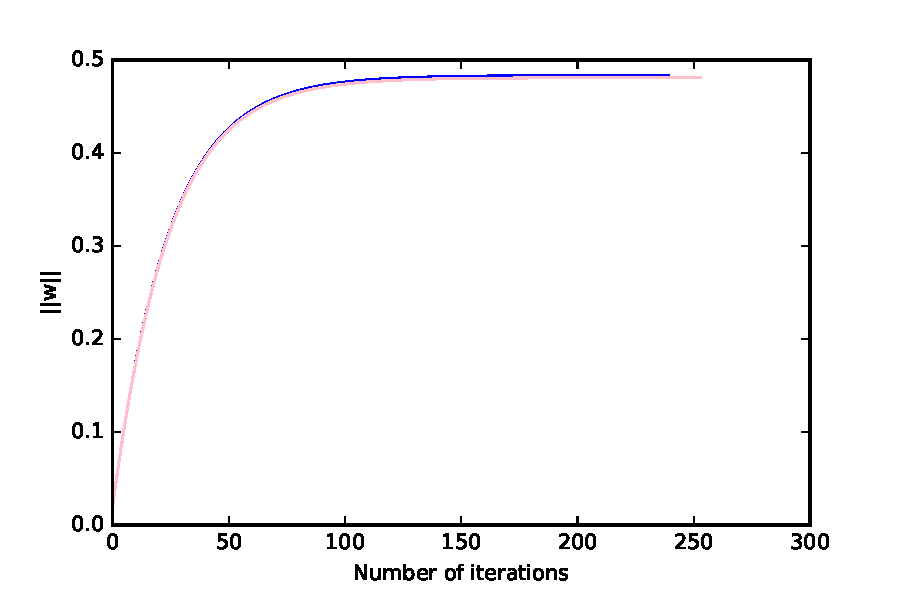
\includegraphics[width=3in]{figures/1-1-weights.pdf}
   \caption{Effects of regularization on weight vector. I promise I'll replace this.}
   \label{fig:weight-regularization}
\end{figure*}

We then compared the effects of $L_1$ and $L_2$ regularization
with Sklearn's \texttt{Logistic Regression} module.  % TODO fix
Recall that the objective function for $L_1$ regularization is
\begin{equation}
    E_{LR}(w, w_0) = \NLL(w, w_0) + \lambda ||w||_1
\end{equation}
where $||w||_1 = \sum_{i=1}^n{|w_i|}$.
We observed that $L_2$ generally produced
more accurate classifications as $\lambda$ increased,
while both resulted similar decision boundaries.
For small $\lambda$,
$L_2$ regularization resulted in smaller weights
than $L_1$ regularization (figure \ref{fig:l1-l2}).

We further tested both regularization methods against four datasets (including the first), each with similar forms of $X$ and $y$ inputs (figure \ref{fig:regularization-four}). Using separate training and validation sets, we determined the optimal regularizer and value of $\lambda$ for each dataset (table \ref{table:regularization-four}).

% TODO and then?

\begin{table*}
\caption{Classification accuracy for logistic regression with $L_2$ and $L_1$ regularization. For each entry, the $L_2$ accuracy is followed by the $L_1$ accuracy. Also piazza says to use cross-validation / model selection stuff but idk what that is D: wasn't in class}
\centering
\begin{tabular}{|c||c|c|c|c|c|c|c|}
\hline
\backslashbox{data}{$\lambda$} & 0.125		& 0.25		 & 0.5	   & 1 & 2 & 4 & 8 \\\hline
1		&  \color{red}1.0, 1.0 &  \color{red}1.0, 1.0 & \color{red}1.0, 1.0 &  \color{red}1.0, 1.0 &   \color{red}1.0, 1.0  & 1.0, 0.995 & 1.0, 0.995 \\
2	& 0.805, 0.805 & 0.805, 0.805 &0.805, 0.805 & 0.805, 0.805 &  0.805,  \color{red}0.81  &  \color{red}0.81, 0.81 &  \color{red}0.81, 0.81 \\
3	& 0.955, 0.95 & 0.96, 0.955 & 0.965, 0.955 & 0.97, 0.955 & 0.97, 0.965 &  0.97,  \color{red}0.975  & 0.97, 0.97\\
4	& 0.4975,  \color{red}0.5 & 0.4975,  \color{red}0.5& 0.4975,  \color{red}0.5& 0.4975,  \color{red}0.5& 0.4975,  \color{red}0.5& 0.4975,  \color{red}0.5& 0.4975,  \color{red}0.5 \\\hline
\end{tabular}
\label{table:regularization-four}
\end{table*}

% % % % % % % % % %
%    PROBLEM 2
% % % % % % % % % %

\section{Support Vector Machines (SVMs)}

\subsection{Dual Soft-SVM}

We implemented the dual form of soft-SVM
with third-party convex optimization software.
Recall that the soft-SVM dual optimization problem takes the form
\begin{equation}
    \label{eq:soft-svm-dual}
    \begin{array}{ll@{}ll}
        \text{maximize}  &\displaystyle -\f{1}{2}\sum_{i,j} \alpha_i \alpha_j y\sind{i} y\sind{j} \angb{x\sind{i}, x\sind{j}}
        +
        \sum_i \alpha_i \\
        \text{subject to}& 0 \le \alpha_i \le C\\
        & \displaystyle\sum_{i=1}^n \alpha_i y\sind{i} = 0
    \end{array}
\end{equation}
for training data $x\sind{i}$
labeled by $y\sind i = \pm 1$.
Hyperparameter~$C$ controls the amount of slack we permit.
Given a new data point $x$,
we predict its label $y$ as
\begin{equation}
    \label{eq:soft-svm-predict}
    y = \sgn\lt(\sum_i \alpha^*_i y\sind{i} \angb{x\sind{i}, x}\rt) \equiv \sgn(t(x))
\end{equation}
where $\alpha^*_i$ is the optimal value of $\alpha_i$
from Equation~\ref{eq:soft-svm-dual}.

For instance, given the sample dataset shown
in Table~\ref{tab:2-1-toy-dataset},
our optimization problem takes the form
\begin{equation}
    \label{eq:soft-svm-dual-concrete}
    \begin{array}{ll@{}ll}
        \text{maximize}  &\displaystyle -\f{1}{2}\alpha^T
        \left[
            \begin{array}{cccc}
                8 & 10 & 2 & 10 \\
                10 & 13 & 3 & 12 \\
                2 & 3 & 1 & 2 \\
                10 & 12 & 2 & 13
            \end{array}
        \right]
        \alpha
        +
        \sum_{i=1}^4 \alpha_i \\
        \text{subject to}& 0 \le \alpha_i \le C\\
        & \alpha_1 + \alpha_2 = \alpha_3 + \alpha_4
    \end{array}
\end{equation}
Upon inspection,
it is clear that for large $C$
(i.e. in the hard-SVM limit),
the support vectors are $(2,2)$ and $(0,-1)$.
% TODO
% include a picture?

\begin{table*}[h]
    \caption{default}
    \begin{center}
    \begin{tabular}{|c|c|c|}
    $x_1$ & $x_2$ & $y$ \\\hline
    2 & 2 & +1 \\
    2 & 3 & +1 \\
    0 & -1 & -1 \\
    -3 & -2 & -1
    \end{tabular}
    \end{center}
    \label{tab:2-1-toy-dataset}
\end{table*}

We tested our soft-SVM implementation
on the same four 2D datasets from the previous section.
% TODO
% makes sure 2D datasets are mentioned in previous section
Setting regularization parameter $C=1$,
% TODO fill in
% mention linearly separable case vs. non-separable

% results
%1 (4/400 support vectors, 0/200 misclassification)
%2 (174/400 support vectors, 36/200 error)
%3 (33/400 support vectors, 6/200 error)
%4 (392/400 sup vec, 122/400 error)



\subsection{Kernelization}

It is often useful to map our raw data
with some nonlinear feature map $\phi$
into a higher dimensional feature space.
However, it is often infeasible to compute and store in memory
all the values $\phi(x\sind{i})$.

Therefore, we recall the ``kernel trick": the insight that
because Equation~\ref{eq:soft-svm-dual} and \ref{eq:soft-svm-predict}
only refer to values $\phi(x\sind{i})$ inside inner products
with other $\phi(x\sind{j})$,
we only need the kernel function
\begin{equation}
    k(x, x') = \angb{\phi\lt(x\rt), \phi\lt(x'\rt)},
\end{equation}
which is usually much easier to compute than the feature map $\phi$.

By replacing the inner products in
Equations~\ref{eq:soft-svm-dual} and \ref{eq:soft-svm-predict}
with the corresponding kernels,
we arrive at the kernelized soft-SVM optimization problem.

We kernelized our SVM routine
and tested it with a linear kernel
\begin{equation}
    k(x, x') = 1 + x\cdot x'
\end{equation}
and with Gaussian RBF kernels
\begin{equation}
    k(x, x') = \exp\lt(-\f{|x - x'|^2}{2\sigma^2}\rt)
\end{equation}
with varying bandwidth~$\sigma$ on the same four datasets as before.  % TODO how did sigma vary?
We chose values of $C$ in
\[
    C \in \{0.01, 0.1, 1, 10, 100\}
\]

% TODO
% Report your results and answer the following questions:



%(a) What happens to the geometric margin 1/|w| as C increases? Will this always happen as we increase C?
Finally, we make some observations about hyperparameter~$C$.
From Equation~\ref{eq:soft-svm-dual},
larger values of $C$ correspond to less tolerance for slack.
So for small $C$,
the model favors
maximizing the margin at the expense of slack,
so we expect increasing $C$ shrinks the geometric margin,
as our experiments also show.
% TODO illustrate?

% (b) What happens to the number of support vectors as C increases?
Consequently, there are fewer support vectors with large $C$:
the margin becomes tighter,
and the model grows increasingly averse to margin errors,
which make up the bulk of the support vectors for small $C$.

%(c)
%The value of C will typically change the resulting classifier
%and therefore also affects the accuracy on test examples.
%Why would maximizing the geometric margin 1/|w|
%on the training set
%not be an appropriate criterion for selecting C?
%Is there an alternative criterion that we could use for this purpose?
The size of the margin
is not a good metric for choosing $C$,
as can make the margin arbitrarily large
by taking $C \to 0$
(indeed, setting $C = 0$ allows arbitrary amounts of slack
with no penalty on the objective function).
We'd instead like a metric that evaluates
the performance of a given $C$
on unseen data.

A better metric for $C$ is
the hinge loss incurred by our classifier
(Equation~\ref{eq:soft-svm-predict} without the $\sgn$ operator)
on a validation dataset:
\begin{equation}
    \sum_{i} \max(0, 1 - y\sind{i} t(x\sind{i}))
\end{equation}
where the sum is taken over all validation data.


% % % % % % % % % %
%    PROBLEM 3
% % % % % % % % % %

\section{SVMs with Pegasos}

% % % % % % % % % %
%    PROBLEM 4
% % % % % % % % % %

\section{MNIST Digit Recognition}


\end{multicols}

\end{document}
